% A simple Line with Grid TiKZ
% Author: Christoph Gerum <gerum@informatik.uni-tuebingen.de>

\documentclass[10pt,a4paper]{article}

\usepackage{tikz}


\begin{document}

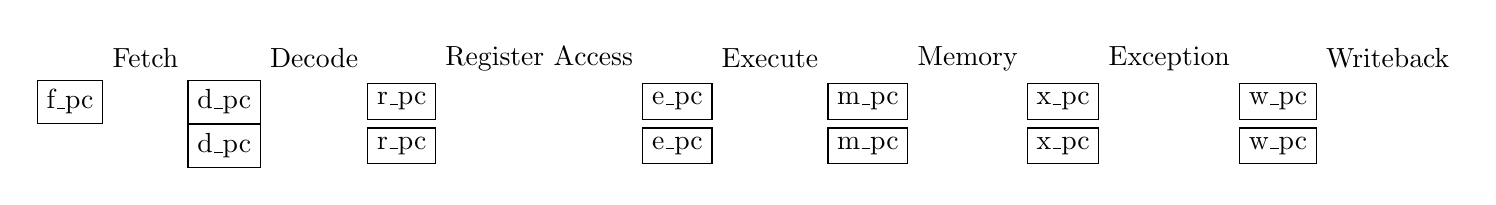
\begin{tikzpicture}[scale=5]

  \matrix{
    & \node(fe){Fetch}; &
    & \node(de){Decode}; &
    & \node(ra){Register Access}; &
    & \node(ex){Execute}; &
    & \node(me){Memory}; &
    & \node(xc){Exception};&
    & \node(wb){Writeback};\\
    \node [draw,shape=rectangle]{f\_pc};&&
    \node [draw,shape=rectangle]{d\_pc};&&
    \node [draw,shape=rectangle]{r\_pc};&&
    \node [draw,shape=rectangle]{e\_pc};&&
    \node [draw,shape=rectangle]{m\_pc};&&
    \node [draw,shape=rectangle]{x\_pc};&&
    \node [draw,shape=rectangle]{w\_pc};\\
    
    &&
    \node [draw,shape=rectangle]{d\_pc};&&
    \node [draw,shape=rectangle]{r\_pc};&&
    \node [draw,shape=rectangle]{e\_pc};&&
    \node [draw,shape=rectangle]{m\_pc};&&
    \node [draw,shape=rectangle]{x\_pc};&&
    \node [draw,shape=rectangle]{w\_pc};\\
  };


\end{tikzpicture}


\end{document}
